\documentclass[11pt]{report}

\usepackage{mathptmx}
\usepackage{url}
\usepackage{graphicx}

\newcommand*{\p}[1]{\textup{\texttt{#1}}}
\newcommand*{\ls}{\textsc{LearnSAT}}
\newcommand*{\pl}{\textsc{Prolog}}
\newcommand*{\sw}{\textsc{SWI-Prolog}}
\newcommand*{\dt}{\textsc{dot}}

\textwidth=16cm
\textheight=22cm
\topmargin=0pt
\headheight=0pt
\oddsidemargin=5mm
\headsep=0pt
\renewcommand{\baselinestretch}{1.1}
\setlength{\parskip}{0.20\baselineskip plus 1pt minus 1pt}
\parindent=0pt

\title{\bfseries \ls\\\mbox{}\\\mbox{}\\
\bfseries\normalsize Version 1.3.2}

\author{\bfseries Mordechai (Moti) Ben-Ari\\\mbox{}\\
\url{http: //www.weizmann.ac.il/sci-tea/benari/}}

%\date{}
\begin{document}

\maketitle

\thispagestyle{empty}

\vspace*{\fill}

\begin{center}
\copyright{} 2012-13 by Mordechai (Moti) Ben-Ari.
\end{center}
This work is licensed under the Creative Commons Attribution-ShareAlike 3.0
License. To view a copy of this license, visit
\url{http://creativecommons.org/licenses/by-sa/3.0/}; or, (b) send a letter
to Creative Commons, 543 Howard Street, 5th Floor, San Francisco,
California, 94105, USA.

\bigskip\bigskip

 
\begin{center}
The following copyright notice applies to the programs described in this
document:\mbox{}\\\mbox{}\\
\copyright{} 2012-13 by Mordechai (Moti) Ben-Ari.
\end{center}

This program is free software; you can redistribute it and/or
modify it under the terms of the GNU General Public License
as published by the Free Software Foundation; either version 2
of the License, or (at your option) any later version.
This program is distributed in the hope that it will be useful
but WITHOUT ANY WARRANTY; without even the implied warranty of
MERCHANTABILITY or FITNESS FOR A PARTICULAR PURPOSE.
See the GNU General Public License for more details.
You should have received a copy of the GNU General Public License
along with this program; if not, write to the Free Software
Foundation, Inc., 59 Temple Place - Suite 330, Boston, MA
02111-1307, USA.

\vspace*{\fill}

\setcounter{tocdepth}{1}
\tableofcontents

\thispagestyle{empty}

\setcounter{page}{0}

\newpage

%%%%%%%%%%%%%%%%%%%%%%%%%%%%%%%%%%%%%%%%%%%%%%%%%%%%%%%%%%%%%%%%%%%%%%%%

\section*{Overview}\addcontentsline{toc}{section}{\textbf{Overview}}

\ls{} is a program for learning about SAT solving. It implements the
classic \emph{Davis-Putnam-Logemann-Loveland (DPLL)} algorithm, together
with modern extensions of the algorithm: \emph{conflict-driven clause
learning (CDCL)} and \emph{non-chronological backtracking (NCB)}.

For a gentle introduction to SAT solvers, see \cite[Chapter~6]{mlcs}.
The comprehensive reference is the \emph{Handbook of Satisfiability}
\cite{SAT}. The algorithms and notation of \ls{} follow \cite{mlm}.

The design of \ls{} is based on the following principles:

\begin{itemize}

\item A very detailed trace of the algorithm's execution is
displayed. The content of the trace can be set by the user.

\item \ls{} is implemented in \pl{} so that the program will be concise
and easy to understand. Only a little knowledge of \pl{} is needed
just to run \ls{}.

\item A utility is provided for converting between sets of clauses
represented as \pl{} terms and those in DIMACS format. While the former
are easier to read, existing formulas in DIMACS format can be used.

\item \ls{} is an open-source project.
\end{itemize}

The three chapters of this document are a user's guide, a tutorial on
SAT solving with \ls{} and documentation of the software.

%%%%%%%%%%%%%%%%%%%%%%%%%%%%%%%%%%%%%%%%%%%%%%%%%%%%%%%%%%%%%%%%%%%%%%%%

\chapter{User's Guide}

\section{Installation}

\ls{} can be downloaded from Google Code at:
\begin{center}
\url{http://code.google.com/p/mlcs/}.
\end{center}

Download and unzip the archive \p{learnsat-N.zip}. The \pl{} source code
is in the directory \p{src} and the documentation is in the directory
\p{docs}.

Download and install \sw{}:\footnote{For possible portability problems,
see Section~\ref{s.port}.}
\begin{center}
\url{http://www.swi-prolog.org/}.
\end{center}
There are binary distributions of \sw{} for Windows and MacOSX.

The source files use the extension \p{pro} instead of the more usual
\p{pl} to avoid conflict with programs in Perl. During the installation
of \sw{}, if you associate the extension \p{pro} with \sw{}, a
program can be launched by double-clicking on its name in a file list. 

The main module is in the file \p{dpll.pro}. It exports the predicates
shown in Table~\ref{tab.export}. These are the only predicates that you
need to run \ls{}.

\begin{table}
\begin{center}
\begin{tabular}{|l|l|}
\hline
\multicolumn{2}{|c|}{\textbf{\large Predicates}}\\
\hline
\p{dpll}&Run the DPLL algorithm\\
\p{usage}&Show the predicates, modes and display options \\
\p{show\_config}&Show the current mode and display options\\
\p{set\_mode}&Set the algorithmic mode\\
\p{set\_display}&Set display options\\
\p{clear\_display}&Clear display options\\
\p{set\_order}&Set variable assignment order\\
\p{clear\_order}&Clear variable assignment order\\
\hline
\end{tabular}
\end{center}
\caption{Predicates exported from the module \p{dpll}}\label{tab.export}
\end{table}


\section{Running \ls}

\subsection{Creating a file to check the satisfiability of a CNF formula}

To check the satisfiability of a CNF formula, create a \pl{} program
that calls the predicate \p{dpll} with the clausal form of the formula
represented as a list of lists of literals.

The file with the program must be in the \p{src} directory;
alternatively, the \ls{} source files can be copied to the directory
that contains that file.

\newpage

Here is a program for the pigeonhole principle for two holes and three
pigeons, where \p{pij} means that pigeon \p{i} is in hole \p{j}:

\begin{verbatim}
:- use_module(dpll).

hole2 :-
  dpll(
  [
  [p11, p12],   [p21, p22],   [p31, p32],   % Each pigeon in hole 1 or 2 
  [~p11, ~p21], [~p11, ~p31], [~p21, ~p31], % No pair is in hole 1
  [~p12, ~p22], [~p12, ~p32], [~p22, ~p32], % No pair is in hole 2
  ], _).
\end{verbatim}

The result (a satisfying assignment or \p{[]} if unsatisfiable) is
returned as the second argument, but can be left anonymous if only
the trace is of interest.

\subsection{Loading and running a file}

Once this file has been loaded (by double-clicking or by consulting
\p{[pigeon]}), the query:
\begin{verbatim}
?- hole2. 
\end{verbatim}

can be run. After it terminates with \p{true} you must press
return to get a new prompt. The output will be a trace of the DPLL
algorithm (Figure~\ref{fig.pigeon}).

\begin{figure}[tbp]
\begin{verbatim}
1 ?- hole2.
LearnSAT v1.3.0. Copyright 2012-13 by Moti Ben-Ari. GNU GPL.
Decision assignment: p11=0
Propagate unit: p12 derived from: 1. [p11,p12]
Propagate unit: ~p22 derived from: 7. [~p12,~p22]
Propagate unit: p21 derived from: 2. [p21,p22]
Propagate unit: ~p31 derived from: 6. [~p21,~p31]
Propagate unit: p32 derived from: 3. [p31,p32]
Conflict clause: 8. [~p12,~p32]
Decision assignment: p11=1
Propagate unit: ~p21 derived from: 4. [~p11,~p21]
Propagate unit: p22 derived from: 2. [p21,p22]
Propagate unit: ~p31 derived from: 5. [~p11,~p31]
Propagate unit: p32 derived from: 3. [p31,p32]
Conflict clause: 9. [~p22,~p32]
Unsatisfiable:
Statistics: clauses=9, variables=6, units=9, decisions=2, conflicts=2
true.
\end{verbatim}
\caption{Running the program for the pigeon-hole principle}\label{fig.pigeon}
\end{figure}

The trace output can be directed to a file:

\begin{verbatim}
?- tell('hole2.txt'), hole2, told.
\end{verbatim}

\newpage

\section{Controlling the algorithms}

\subsection{Choosing the algorithmic mode}

\ls{} can run in one of three modes set by the predicate \p{set\_mode}
(Table~\ref{tab.modes}).

\begin{table}[*hb]
\begin{center}
\begin{tabular}{|l|l|}
\hline
\multicolumn{2}{|c|}{\textbf{\large Modes}}\\
\hline
\p{dpll} & DPLL algorithm (default)\\
\p{cdcl} & DPLL with conflict-directed clause learning\\
\p{ncb} &  DPLL with CDCL and non-chronological backtracking\\
\hline
\end{tabular}
\caption{\ls{} modes}\label{tab.modes}
\end{center}
\end{table}


For the three-layer grid-pebbling problem, the statistics for the three
modes are:
\begin{verbatim}
         dpll: units=74, decisions=50, conflicts=26
         cdcl: units=25, decisions=14, conflicts=8
         ncb:  units=17, decisions=9,  conflicts=3
\end{verbatim}

\subsection{Order of variable assignment}

By default, decision assignments are made in lexicographical order of
the atomic propositions. The order can be specified by using the
predicate \p{set\_order}; the predicate \p{clear\_order} resets the
default order. The list argument to \p{set\_order} must be a permutation
of the variables in the clauses.\footnote{Suggestion: First run a
program with the display option \p{variable} set; the list of variables
will be printed out in the correct syntax for \p{set\_order}. You can
now copy and paste list, permutating the order as needed.} Negated
variables can be given; these variables are assigned 1 before they are
assigned 0.

The \p{mlm} example finds a satisfying assignment \emph{without}
conflicts if the default order is changed:

\begin{verbatim}
     set_order([x1,x2,x021,x031,x3,x4,x5,x6]).
\end{verbatim}

\section{Tracing the algorithms}

\subsection{Display options}

\ls{} writes extensive trace output as it executes the algorithms. Each
line starts with a string followed by a colon to make it easy to
postprocess the output. The content of the trace is controlled using
\p{set\_display} and \p{clear\_display}. The argument to these
predicates can be \p{all} or \p{default} or a single option or a list of
options taken from Table~\ref{tab.display}, where * denotes the default
options.

The options \p{literal} and \p{uip} are relevant only if \p{resolvent}
is also selected. Selecting the incremental implications graphs also
selects the final graphs.

In \p{cdcl} and \p{ncb} modes, the assignments are written together with
their levels in the format \p{p1=0@3} used in \cite{mlm}.
By selecting \p{antecedent}, the antecedent clause can be displayed with
assignment forced by unit propagation:
\verb+p1@3/[~p1,p3]+.

If you need to change the mode and options frequently, you
can write a predicate to do so:
\begin{verbatim}
ncb_mode :-
  set_mode(ncb),
  set_display(default),
  set_display([antecedent, graph]).
\end{verbatim}

\begin{table}[tbp]
\begin{center}
\begin{tabular}{|l|l|}
\hline
\multicolumn{2}{|c|}{\textbf{\large Display options}}\\
\hline
\p{antecedents}&  antecedents of the implied literals\\
\p{assignments}& assignments that caused a conflict         \\
\p{backtrack} *&  level of non-chronological backtracking    \\
\p{clauses}   &  clauses to be checked for satisfiability   \\
\p{conflict} * &  conflict clauses                           \\
\p{decision} * &  decision assignments                       \\
\p{dominator} &  learned clause computed from a dominator   \\
\p{dot}       &  implication graphs (final) in dot format           \\
\p{dot\_inc}  &  implication graphs (incremental) in dot format\\
\p{evaluate}  &  evaluation of clauses for an assignment    \\
\p{graph}     &  implication graphs (final)                 \\
\p{incremental}& implication graphs (incremental)           \\
\p{label}     &  graph labeled with clauses, not just numbers\\
\p{learned} *  &  learned clauses                            \\
\p{literal}   &  literals found assigned during CDCL        \\
\p{partial}   &  partial assignment so far                  \\
\p{resolvent} * &  resolvents created during CDCL             \\
\p{result} *   &  result of the algorithm with statistics    \\
\p{skipped} *  &  assignments skipped when backtracking      \\
\p{sorted} *   & assignments displayed in sorted order\\
\p{tree}       &  assignment tree in dot format\\
\p{tree\_inc}  &  assignment tree (incremental) in dot format\\
\p{uip} *       &  unique implication points                  \\
\p{unit} *     &  unit clauses                               \\
\p{variables} &  variables that are not assigned so far     \\
\hline
\end{tabular}
\end{center}
\caption{Display options}\label{tab.display}
\end{table}

\clearpage

\section{Graphical output}

\subsection{Implication graphs}\label{s.impl}

When a conflict clause is encountered, \ls{} generates the implication
graph, both the final graph and the graphs that are incrementally
generated. A graph is shown in the tutorial below
(Figure~\ref{fig.graph}). The graphs can be displayed in the trace
(display options \p{graph} and \p{incremental}) and they can be written
to a file (display options \p{dot} and \p{dot\_inc}) in \dt{} format
which can be rendered using
\textsc{GraphViz}:\footnote{\url{http://www.graphviz.org/}.}

\begin{verbatim}
dot -Tpng examples-ig-00.dot > examples-ig-00.png
\end{verbatim}

If the display option \p{label} is selected, the edges are labeled with
the clauses and not just their numbers.

A script can run \dt{} on all the files of the incremental graphs; in
Windows, the batch command is:

\begin{verbatim}
for %%F in (*.dot) do c:\"program files"\graphviz\bin\dot -Tpng %%F > %%~nF.png
\end{verbatim}


\subsection{Assignment trees}

The Assignment trees showing the sequences of assignments to variables
can be generated by selecting \p{tree}
(Figure~\ref{fig.tree1}--\ref{fig.tree3}). Trees are shown as directed
acyclic graphs whose nodes are assignments rather than variables. There
is a separate tree for each new assignment, whether a decision
assignment or an implied assignment. The former are decorated with a red
border. Conflict nodes are decorated with a double red border and a
double green border indicates the node (if any) that causes the formula
to become satisfiable.

The rendering of the \dt{} files is as described above for the
implication graphs.

\section{Configuration}


The version, the default and current mode, and the default and
current display options can be shown by running \p{show\_config}.

The file \p{config.pro} can be edited to change: the default mode and
display options and---for the implication graphs and assignment
trees---the \dt{} prologue and the decoration of the decision nodes.


\newpage


\section{Test programs included in \ls{}}

\begin{itemize}
\item \p{examples.pro}: Examples from papers on SAT
solvers \cite{mz,mlm,ms}.

\item \p{tseitin.pro}: Tseitin clauses for $K_{2,2}$,
$K_{3,3}$ and the example from \cite[Section 4.5]{mlcs}.

\item \p{queens.pro}: The 4-queens problem.

\item \p{pigeon.pro}: The pigeon-hole principle for 2 and 3 holes.

\item \p{pebbles.pro}: Grid pebbling for 2 and 3 layers.
\end{itemize}

\section{DIMACS transformation}

The predicates in \p{dimacs.pro} convert a set of clauses in
\pl{} format (a list of lists of literals) to and from \emph{DIMACS cnf
format}:
\begin{itemize}
\item \p{to\_dimacs(File, Comment, Clauses)} converts the \pl{}
\p{Clauses} into DIMACS format and writes them to the \p{File} with the
\p{Comment}.
\item \p{from\_dimacs(Predicate, InFile, OutFile)} reads \p{InFile} in
DIMACS format; the \pl{} format to run \p{dpll} is written to
\p{OutFile}:
\begin{verbatim}
Predicate :- dpll(List, _).
\end{verbatim}
\end{itemize}

%%%%%%%%%%%%%%%%%%%%%%%%%%%%%%%%%%%%%%%%%%%%%%%%%%%%%%%%%%%%%%%%%%%%%%%%

\chapter{Tutorial}

\section{The DPLL algorithm}

For the tutorial, we will use the set of clauses from \cite{mlm} as our
example:\footnote{The file \p{examples.pro} contains the predicate
\p{mlm} that runs \p{dpll} on this set of clauses. Since \ls{} tries
decision assignments in lexicographic order, two literals have a \p{0}
added to their names to ensure that they are chosen as in \cite{mlm}.}

\begin{verbatim}
  1. [x1,x031,~x2]   2. [x1,~x3]         3. [x2,x3,x4]
  4. [~x4,~x5]       5. [x021,~x4,~x6]   6. [x5,x6]
\end{verbatim}

When the DPLL algorithm is applied to the set of clauses, it assigns
0 to \p{x021}, \p{x031} and \p{x1}:

\begin{verbatim}
?- mlm.
LearnSAT v1.2.0. Copyright 2012 by Moti Ben-Ari. GNU GPL.
Decision assignment: x021=0
Decision assignment: x031=0
Decision assignment: x1=0
\end{verbatim}

Clause 1 is now a unit clause implying that \p{x2} must be assigned 0
and clause 2 is also a unit clause implying that \p{x3} must be assigned
0. This in turn leads to a sequence of unit propagations until clause 6
is falsified:

\begin{verbatim}
Propagate unit: ~x2 derived from: 1. [x1,x031,~x2]
Propagate unit: ~x3 derived from: 2. [x1,~x3]
Propagate unit: x4 derived from: 3. [x2,x3,x4]
Propagate unit: ~x5 derived from: 4. [~x4,~x5]
Propagate unit: ~x6 derived from: 5. [x021,~x4,~x6]
Conflict clause: 6. [x5,x6]
\end{verbatim}

\pagebreak[3]

The algorithm backtracks, trying the assignment of 1 to \p{x1} and then
0 to \p{x2} and \p{x3}:
\begin{verbatim}
Decision assignment: x1=1
Decision assignment: x2=0
Decision assignment: x3=0
\end{verbatim}
which causes another sequence of unit propagations leading to the same
conflict clause:
\begin{verbatim}
Propagate unit: x4 derived from: 3. [x2,x3,x4]
Propagate unit: ~x5 derived from: 4. [~x4,~x5]
Propagate unit: ~x6 derived from: 5. [x021,~x4,~x6]
Conflict clause: 6. [x5,x6]
\end{verbatim}

The algorithms backtracks to assign 1 to \p{x3}, followed by 0 to \p{x4}
and \p{x5}, and the propagation of a unit; the result is a set of
assignments that satisfies the set of clauses:
\begin{verbatim}
Decision assignment: x3=1
Decision assignment: x4=0
Decision assignment: x5=0
Propagate unit: x6 derived from: 6. [x5,x6]
Satisfying assignments:
[x021=0,x031=0,x1=1,x2=0,x3=1,x4=0,x5=0,x6=1]
Statistics: clauses=6, variables=8, units=9, decisions=9, conflicts=2
\end{verbatim}

\section{Assignment trees}

The assignment trees are shown in 
Figures~\ref{fig.tree1}--\ref{fig.tree3}. In DPLL mode, backtracking is
to the most recent decision mode and evaluation and unit propagation
proceed normally. In CDCL mode, backtracking is the same but the
satisfying assignment without additional decisions because of the effect
of the learned clause. In NCB mode, backtracking is to the first
decision node. The antecedent clause is shown in addition to the
assignments for non-decision nodes.

\begin{figure}
\begin{center}
\includegraphics[keepaspectratio=true,width=.9\textwidth]{tree1}
\caption{Assignment tree in DPLL mode}\label{fig.tree1}

\bigskip
\bigskip
\bigskip

\includegraphics[keepaspectratio=true,width=.9\textwidth]{tree2}
\caption{Assignment tree in CDCL mode}\label{fig.tree2}

\bigskip
\bigskip
\bigskip

\includegraphics[keepaspectratio=true,width=.9\textwidth]{tree3}
\end{center}
\caption{Assignment tree in NCB mode}\label{fig.tree3}
\end{figure}

\clearpage

\section{Conflict-driven clause learning}

Let us now run the same example with CDCL after first setting the mode
and display options:

\begin{verbatim}
?- set_mode(cdcl).
?- set_display([literal, dot, graph]).
?- mlm.
\end{verbatim}

\subsection{The implication graph}

When the conflict clause is found the \emph{implication graph} is
generated (Figure~\ref{fig.graph}). It represents the result of unit
propagation that causes a conflict. There are three source nodes, one
for each of the decision assignments (\p{x021=0@1}, \p{x031=0@2},
\p{x1=0@3}) that are sufficient to cause a conflict by unit propagation.
The level of each decision assignment is added to the assignment in
\p{cdcl} mode.

The conflict is represented by the sink node \p{kappa} and the
assignments that were forced by unit propagation are represented by
nodes labeled with the assignments. An edge of the graph is labeled with
the number of the clause that is the \emph{antecedent} of the node; this
is the unit clause that forced the assignment labeling that node. The
display option \p{label} will display the clause itself in addition to
its number, as shown in Figure~\ref{fig.graph}. There is an edge for
each literal in the unit clause (except the one whose assignment is
forced) and the sources of these edges are the assignments to those
literals. For example, the decision assignments \p{x1=0@3}, \p{x031=0@2}
cause clause 1 \verb+[x1, x031, ~x2]+ to become a unit clause and force
the assignment of 0 to \p{x2}. A node labeled \p{x2=0@3} is added to the
graph together with edges labeled clause 1 from the nodes for the
decision assignments.

\begin{figure}
\begin{center}
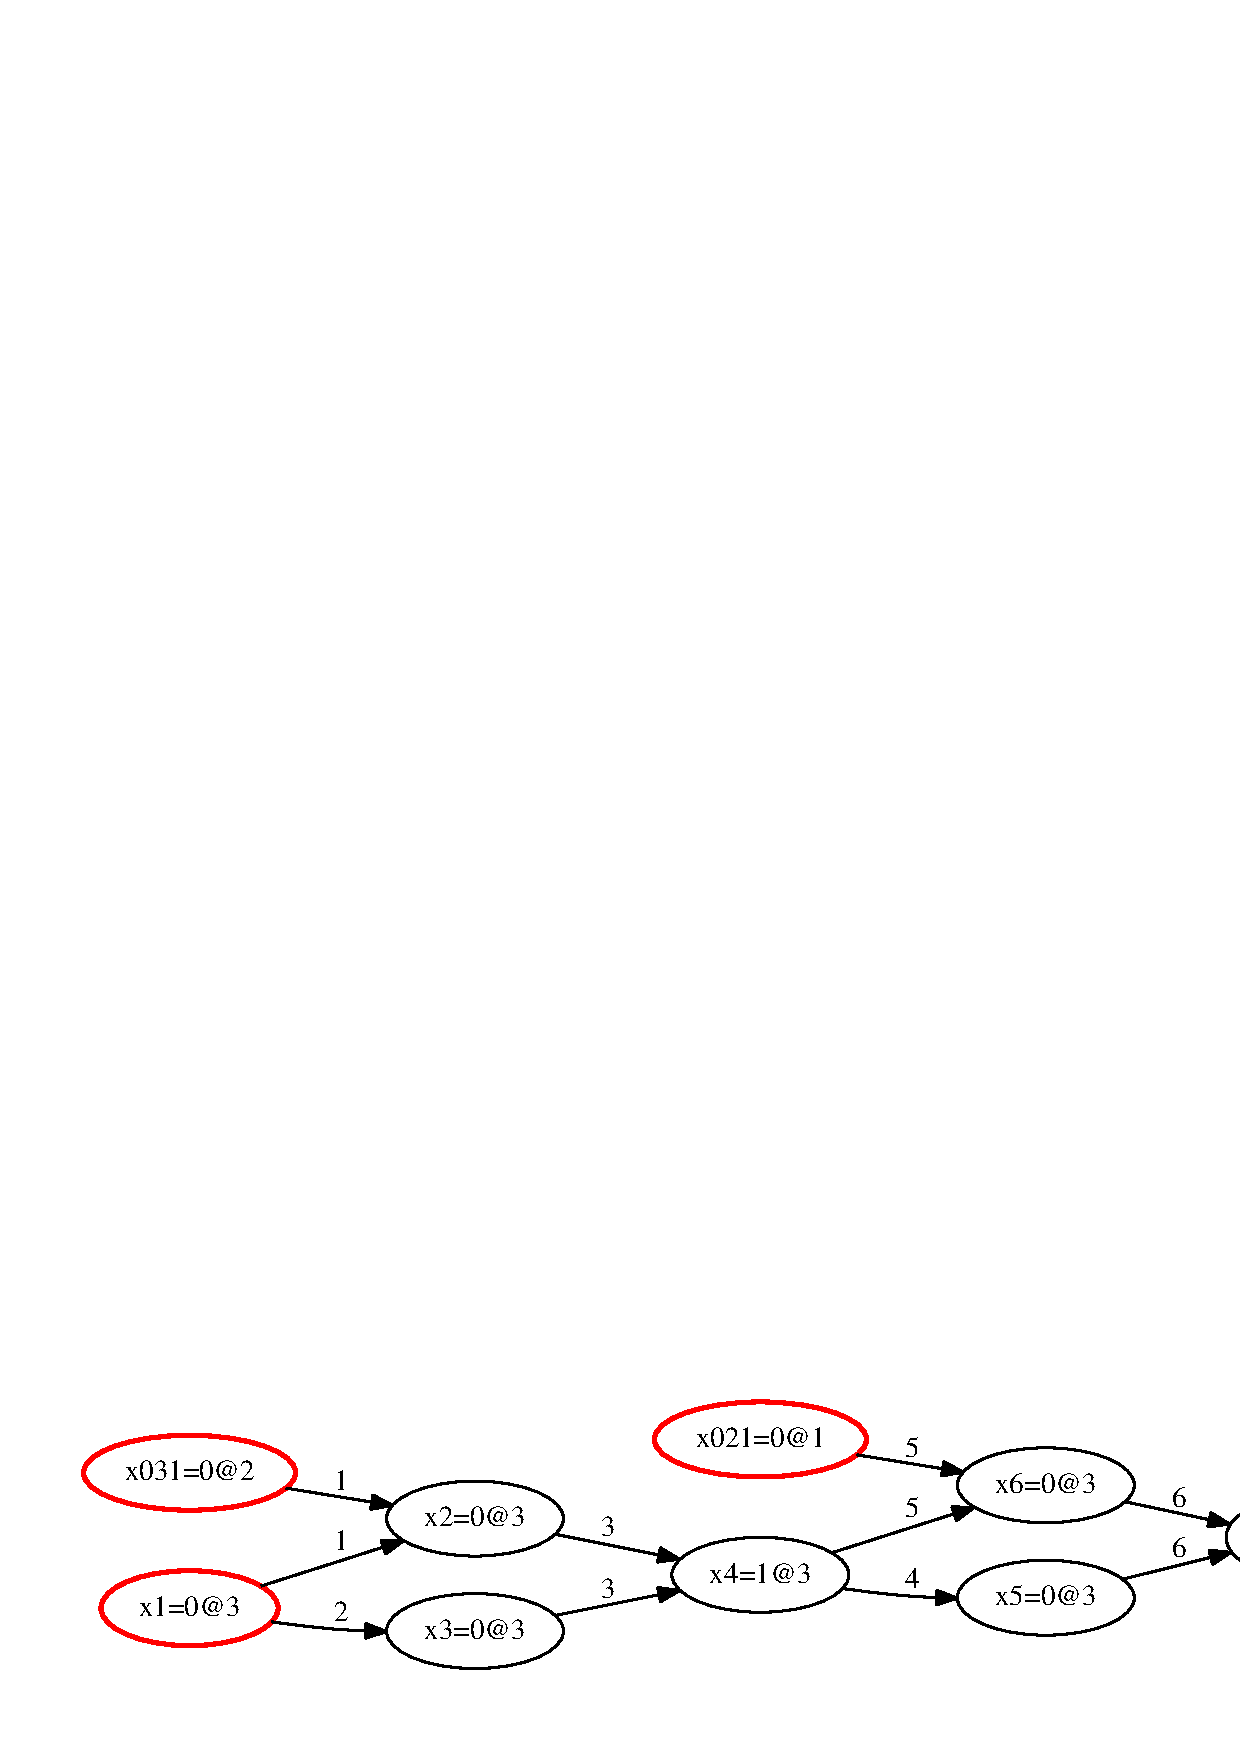
\includegraphics[keepaspectratio=true,width=\textwidth]{graph}
\end{center}
\caption{Implication graph}\label{fig.graph}
\end{figure}

\subsection{Learning a clause from dominators}

Learning the clause \p{[x021, x031, x1]} defined by the complements of
the decision assignments will ensure that this unit propagation is never
done again because the clause will immediately be falsified.
However, a better clause to learn can be computed as follows. 

Consider all the (four) paths from the \emph{last} decision assignment
\p{x1=0@3} to the kappa node. A node (here, the node \p{x4=1@3}) is
called a \emph{dominator} if it appears on all the paths. A dominator is
a \emph{unique implication point (UIP)} because its assignment
participates in the conflict in the same way as do \emph{all} the
decision assignments that it dominates. Here, the assignment \p{x4=1@3}
is implied by \p{x031=0@2} and \p{x1=0@3}, so \p{x4} can replace
\p{x031} and \p{x1} in the learned clause. To display the generation of
the learned clause, select the display option \p{dominator}:

\begin{verbatim}
Paths from the decision node at this level to kappa:
x1=0@3 --> x2=0@3 --> x4=1@3 --> x5=0@3 --> kappa
x1=0@3 --> x2=0@3 --> x4=1@3 --> x6=0@3 --> kappa
x1=0@3 --> x3=0@3 --> x4=1@3 --> x5=0@3 --> kappa
x1=0@3 --> x3=0@3 --> x4=1@3 --> x6=0@3 --> kappa
A dominator is: x4=1@3
Decisions at a lower level: [assign(x021,0,1,yes),assign(x031,0,2,yes)]
Decisions not dominated: [assign(x021,0,1,yes)]
Learned clause from dominator: [x021,~x4]
\end{verbatim}

This method of learning a clause is performed \emph{only for display
purposes} if the display option \p{dominator} is selected. The learned
clause that is used is determined by a different method described in the
next subsection.

\subsection{Learning a clause by resolution}

The conflict clause (the antecedent clause of the \p{kappa} node) is
defined as the \emph{current clause} and resolution is carried out until
a UIP is found. The clause to be resolved with the current clause at
each step is one that clashes with the current clause on a literal that
is assigned at the current level \emph{by unit propagation}. For
example, given the current (conflict) clause \p{[x5,x6]}, \p{x5} was
assigned by unit propagation at this level, so we can resolve
\p{[x5,x6]} with the antecedent clause \verb+[~x4,~x5]+ to obtain the
resolvent \verb+[~x4,x6]+ which becomes the current clause. The next
step is to resolve this clause with \verb+[x021,~x4,~x6]+ to obtain
\verb+[x021,~x4]+. The resolution now terminates
because clause is a UIP, namely, a clause where only one literal is
assigned at the current level. The \ls{} output is:

\begin{verbatim}
Literal: x5 assigned at level: 3
Literal: x6 assigned at level: 3
Not a UIP: two literals are assigned at level: 3
Clause: [x5,x6] unsatisfied
Complement of: x5 assigned true in the unit clause: [~x4,~x5]
Resolvent of the two clauses: [x6,~x4] is also unsatisfiable
Literal: x6 assigned at level: 3
Literal: ~x4 assigned at level: 3
Not a UIP: two literals are assigned at level: 3
Clause: [x6,~x4] unsatisfied
Complement of: x6 assigned true in the unit clause: [x021,~x4,~x6]
Resolvent of the two clauses: [x021,~x4] is also unsatisfiable
Literal: ~x4 assigned at level: 3
UIP: one literal is assigned at level: 3
Learned clause: [x021,~x4]
\end{verbatim}

The DPLL algorithm now continues as before but with the learned clause
added to the set of clauses. The result is that a satisfying assignment
is found more efficiently with fewer decisions (6 instead of 9):

\begin{verbatim}
Decision assignment: x1=1@3
Propagate unit: ~x4 derived from: 7. [x021,~x4]
Decision assignment: x2=0@4
Propagate unit: x3 derived from: 3. [x2,x3,x4]
Decision assignment: x5=0@5
Propagate unit: x6 derived from: 6. [x5,x6]
Satisfying assignments:
[x021=0@1,x031=0@2,x1=1@3,x2=0@4, x3=1@4,x4=0@3,x5=0@5,x6=1@5]
Statistics: clauses=6, variables=8, units=8, decisions=6, conflicts=1
\end{verbatim}

\section{Non-chronological backtracking}

Let us now select the NCB mode:
\begin{verbatim}
?- set_mode(ncb).
?- mlm.
\end{verbatim}

When a learned clause has been obtained, the backtrack level for
non-chronological backtracking is computed. This is the highest level of
an assignment in the learned clause except for the current level.
The DPLL algorithm skips decision assignments whose level is at a lower
level than the backtrack level. In the example, the highest level is 1
where \p{x021} was assigned:

\begin{verbatim}
Non-chronological backtracking to level: 1
Skip decision assignment: x1=1@3
Skip decision assignment: x031=1@2
\end{verbatim}

For this example, there is no difference between CDCL with and without
NCB, but for the three-hole pigeonhole principle, the difference is
significant:
\begin{verbatim}
Statistics: clauses=22, variables=12, units=243, decisions=96, conflicts=91

Statistics: clauses=22, variables=12, units=105, decisions=34, conflicts=26
\end{verbatim}

%%%%%%%%%%%%%%%%%%%%%%%%%%%%%%%%%%%%%%%%%%%%%%%%%%%%%%%%%%%%%%%%%%%%%%%%

\chapter{Software documentation}

\section{Module structure}

The \ls{} software consists of the following source files:\footnote{The
list does not including the test programs and the program for DIMACS
conversion.}

\begin{itemize}
\item \p{dpll.pro}: Main module for the DPLL algorithms.\\

\item \p{auxpred.pro}: Auxiliary predicates for the DPLL algorithms. 

\item \p{io.pro}: Predicates for writing assignments, clauses and
implication graphs.

\item \p{display.pro}: Display the trace using predicates \p{display/n},
where the first argument is a display option and the additional
arguments supply the data to be displayed.

\item \p{config.pro}: Default configuration data. The module contains
the facts: \p{version}, \p{years}, \p{default\_mode},
\p{default\_display}, \p{dot\_prologue}, \p{dot\_decorate}.

\item \p{counters.pro}: Maintains and displays counters for units,
decisions and conflicts. Stores the number of clauses and variables for
printing the statistics. Defines a counter for adding a number to the
file names for implication graphs.

\item \p{modes.pro}: Sets, clears and checks the mode and the display
options. It also implements \p{usage} and \p{show\_config}. The dummy
display option \p{none} is used to distinguish between the initial state
(no options, so set the default options) and a state where all options
have been cleared.

\item \p{dominator.pro}: Computing dominators in the implication graph. 

\item \p{dot.pro}: Generating the \dt{} files of the implication graphs
and the assignment trees.
\end{itemize}

\newpage

\section{Data structures}

The following dynamic predicates are used:
\begin{itemize}
\item In \p{dpll.pro}: The non-chronological backtracking level (an
 integer) is stored in the predicate \p{backtrack}.

\item In \p{dpll.pro}: The learned clauses are stored as a list of
clauses in the predicate \p{learned}.

\item In \p{auxpred.pro}: If the user specifies the order of assignment
to variables, the list is stored in \p{variables\_list}.

\item In \p{dot.pro}: \p{node} and \p{edge} are used when building the
assignment trees. They store the paths leading to previous conflict
nodes and are updated with each new path.

\item In \p{mode.pro}: The current mode and display options are stored
in \p{mode} and \p{display\_option}. 

\end{itemize}

Two functors are used to create terms:
\begin{itemize}

\item \p{assign} represents an assignment and takes four arguments: a
variable, its value and level and \p{yes} if this is a decision
assignment or the antecedent clause of an implied assignment.

\item \p{graph} is an implication graph. Its arguments are a list of
nodes which are assignments and a list of edges which are terms with
functor \p{edge} and three arguments: the source and target nodes
and the clause that labels the edge.
\end{itemize}


\section{The DPLL algorithm}

The predicate \p{dpll/2} implements the DPLL algorithm on a set of
clauses represented as a list of lists of literals. It returns a list of
satisfying assignments or the empty list if the clauses are
unsatisfiable. As part of its initialization, the set of variables in
the clauses is obtained from the list.

The predicate \p{dpll/2} invokes \p{dpll/6} which is the main recursive
predicate for performing the algorithm. If the set of variables to be
assigned to is empty, the set of clauses is satisfiable. Otherwise,
\p{dpll/6} tries to perform unit propagation by searching for a unit and
then evaluating the set of clauses. When no more units remain, it
chooses a decision assignment and evaluates the set of clauses.

The predicate \p{ok\_or\_conflict} is called with the result of the
evaluation of unit propagation or the choice of an assignment. If the
result is not a conflict clause, the variable chosen is deleted and
\p{dpll/6} is called recursively. If there was a conflict clause, the
implication graph is constructed and a learned clause is generated from
the graph; then \p{ok\_or\_conflict} fails so that backtracking can try
a new assignment.

The predicate \p{evaluate} receives a set of clauses and evaluates them,
returning \p{ok} or \p{conflict}. For each clause it calls
\p{evaluate\_clause}, which returns \p{satisfied}, \p{unsatisfied},
\p{unit} or \p{unresolved}.

\p{find\_unit} traverses the list of clauses using the current
assignments. It calls \p{evaluate\_clause} on each clause and succeeds
if that predicate returns \p{unit}.

\p{choose\_assignment} returns an assignment. \emph{Condition}
$\rightarrow$ \emph{Action} with an internal \p{!, fail} implements
non-chronological backtracing. (See Section~4.7 of the \sw{} Reference
Manual for the meaning of a cut within this construct.)


\section{CDCL and NCB}

The implication graph is built incrementally. Whenever a unit clause is
found, \p{extend\_graph} is called with the unit clause, its number (to
label the new edges), the assignment it implies (to create the new
target of the edges) and the graph constructed so far. For each literal
(except the one implied), a new edge is created and when the list of
literals has been traversed, the new node is created. When a conflict is
encountered, the \p{kappa} node and its incoming edges are added and the
graph is passed to \p{compute\_learned\_clause\_by\_resolution}.

\p{compute\_learned\_clause\_by\_dominator} computes a learned clause by
locating a dominator of the highest-level decision assignment node
relative to the \p{kappa} node. \p{findall} with \p{get\_path} returns a
list of all paths from the decision node to the \p{kappa} node. This
list is an argument to \p{get\_dominator} which finds a node that
appears on all the paths. \p{findall} with
\p{lower\_decision\_assignment} creates a list of all decision nodes at
lower levels and then \p{findall} is called with \p{no\_path} to extract
those nodes with no path to the dominator. The learned clause is the
complement of the assignment at the dominator, together with the
complements of decision assignments labeling nodes that are not
dominated.

The predicate \p{compute\_learned\_clause\_by\_resolution} starts with
the conflict clause (the antecedent clause of the \p{kappa} node) as the
current clause. In \p{compute\_learned\_clause}, a search is made for a
clause that contains the complement of a literal in the current clause
and which is assigned at the current level by unit propagation, that is,
it is not a decision node. \p{resolve} computes the resolvent of the two
clauses and \p{compute\_learned\_clause} is called with the resolvent as
the new current clause. The resolution terminates when \p{check\_uip}
identifies the current clauses as a UIP. This clause is the learned
clause and the predicate \p{compute\_learned\_clause\_by\_resolution}
adds it to the list that is the argument of the fact \p{learned}.

When a learned clause has been obtained, \p{compute\_backtrack\_level}
returns the highest level of an assignment in the learned clause except
for the current level.


\section{Auxiliary predicates}\label{s.aux}

\begin{itemize}

\item \p{is\_assigned} checks if a literal has been assigned a value
and if so returns that value.

\item \p{literals\_to\_variables} takes a list of literals and returns a
sorted set of the variables corresponding to the literals.

\item \p{to\_variable} returns the variable of a literal;
\p{to\_complement} returns the complement of a literal.

\item \p{to\_assignment} and \p{to\_literal} convert to and from a
literal and an assignment expressed as a term \p{assign(Variable, Value,
Level, Decision)}.

\end{itemize}


\section{Portability}\label{s.port}

\ls{} was developed on \sw{} but an effort was made to use only portable
constructs. The possible exceptions are:

\begin{itemize}
\item Modules: \p{module}, \p{use\_module}, \p{reexport}.
\item The following predicate to obtain the file name from the command
line:
\begin{verbatim}
  current_prolog_flag(argv, [_, File | _])
\end{verbatim}
\end{itemize}

\bibliographystyle{plain}
\bibliography{learnsat}
\end{document}
